
\chapter{Implementation}
\textit{This chapter outlines the specifications of the hardware platform to be used for flight testing. The state estimation algorithms developed in the previous chapter are now tested using sensor data from a number of flight tests. }


\section{Hardware}\label{section:Hardware}
%Verify EKF using Hardware
%Description of the Hardware
%Pixhawk 2.1 CubeBlack, Intel Edison, APSync, Ardupilot ArduCopter 4.1. 
%Sensors onboard the Cube, plus OFS and GPS external sensors.

In addition to the simulation results, test flights were conducted with a custom hexacopter with the aim of collecting data to verify the EKF algorithm. The hexacopter frame is based upon a commercially available kit known as the Storm Drone 6, along with a custom PCB structure for power distribution. Power is supplied by a 5500 mAh 3S Lithium Polymer (LiPo) battery with a nominal voltage of 11.1 V. The battery voltage is regulated at 5 V to supply the flight controller. The propellers are driven by 1260 kv brushless DC motors. The speed of the motors is controlled by a PWM signal supplied to the associated electronic speed controllers (ESC).

\subsection{The Cube Autopilot}
The drone is controlled by a commercial flight controller known as The Cube Autopilot (formerly known as Pixhawk 2.1). The Cube runs a 32-bit STM32F427 ARM Cortex M4 core, has 256 kB of RAM and 2 MB of flash. It also has a co-processor (STM32F103), which handles failure conditions. It has a number of connectivity options for peripherals (e.g. UART, I2C, CAN buses), as well as 14 pulse width modulation (PWM) outputs for interfacing with actuators. This platform also has a microSD card slot for storage of flight data logs.
\subsection{ArduPilot Software}
The vehicle is controlled using the open source flight software Ardupilot, with the specific version being ArduCopter 4.1. The flight software is run on a Linux-based real-time operating system (RTOS) known as ChibiOS. The code base is mostly written in C++. State estimation is performed via an EKF-based algorithm. The control system is uses cascaded PID control similar to the controller developed in Section \ref{section:PIDControl}. There are also a number of flight modes which are able to be selected for various purposes, i.e. for autonomous flight or radio-controlled flight.

\subsection{Companion Computer}
Additionally, a computer-on-module known as the Intel Edison was added to the Cube flight controller in order to enhance the system capabilities and enable wireless communication. The Edison has a 500 MHz dual-core processor, 1 GB RAM, 4 GB storage and dual-band (2.4 and 5 GHz) WiFi connectivity. The Edison is connected via a designated 70-pin Hirose DF40 connector inside the case of the Cube. Communication with the ArduPilot software is via the MAVLink communication protocol.

APSync, an open source software package developed for use with ArduPilot, was installed on the Edison. This included a Linux operating system as well as a number of python and DroneKit packages. DroneKit is an open source API which allows python scripts to be run on flight control hardware. The relationship between the different systems is shown in \figref{fig:ArduArch}.

\begin{figure}[htb]
\begin{center}
	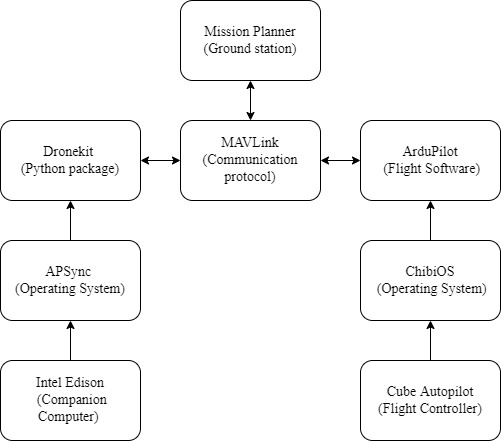
\includegraphics[width=80mm]{ArduPilotArchitecture.jpg}%
	\end{center}
	\caption{System hardware, software and firmware interconnections.}%	
	\label{fig:ArduArch}
\end{figure}

\FloatBarrier
\subsection{Sensors}
The Cube flight controller contains three sets of IMUs (accelerometer, gyroscope and magnetometer), two of which are mechanically vibration-isolated. Two of the IMUs are the Invensense MPU9250 and the third is made up of the STM LSM303D (accelerometer and magnetometer) and L3GD20 (gyroscope). The Cube also contains two barometers, both of which are the MS5611. Multiple of each kind of sensor are provided for redundancy and the EKF in the ArduPilot firmware fuses the data from all sensors for additional accuracy.

Additional sensors were connected to the Cube Autopilot system to enable the previously developed EKFs to be tested.  

A Ublox NEO-M8N GPS module was connected to provide positional data. This module also houses a magnetometer for additional external measurement of the Earth's magnetic field. The GPS module communicates with the flight controller via the I2C protocol.


An integrated optical flow and lidar sensor, Matek 3901-L0X, was also connected to the system. This module consists of a Pimoroni PMW3901 optical flow sensor, an Adafruit VL53L0X lidar sensor and a STM32L051 microcontroller, as well as additional power regulating circuitry. This sensor is able to communicate over UART using Multiwii Serial Protocol (MSP), which is supported by the ArduPilot firmware.

\begin{figure}[htb]
	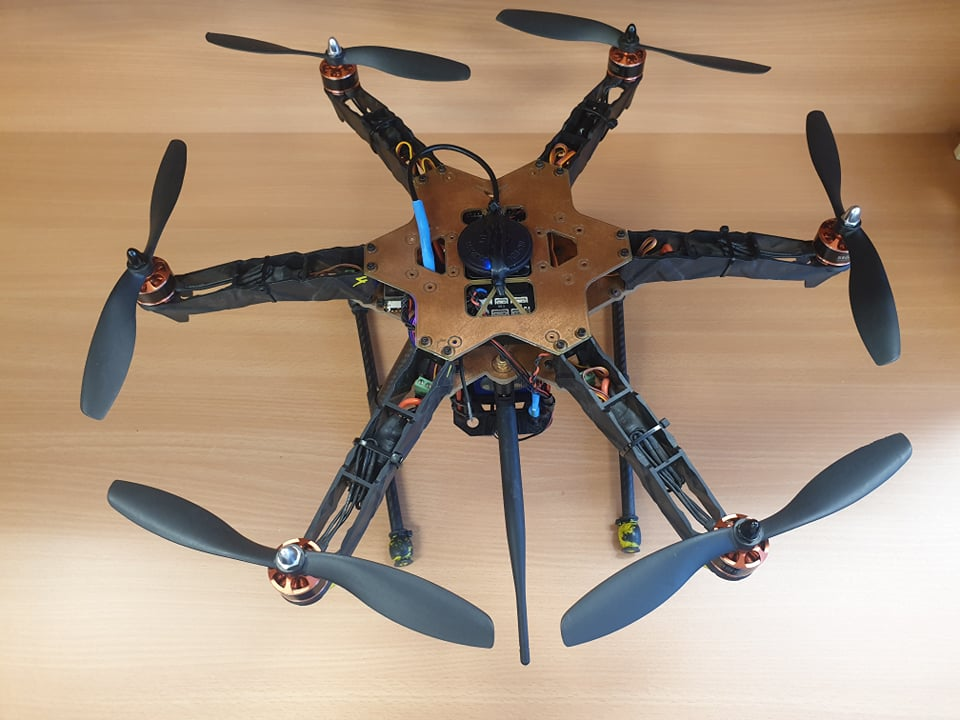
\includegraphics[width=\columnwidth]{Hexacopter_Hardware.jpg}%
	\caption{Hardware platform used for flight testing.}%
	\label{fig:hardware}%
\end{figure}

\FloatBarrier
\subsection{Flight Testing}
Flight testing was conducted by programming the hexacopter with an autonomous mission, which involved taking off to a height of 1.5 metres, travelling approximately 11 metres to a second position and landing. The drone performed the mission successfully using the ArduPilot flight control software and the sensor data recorded during the flight was logged to the onboard SD card. This data was processed in MATLAB and used with the EKF algorithm described in Section \ref{section:GPS_EKF}. \figref{fig:HW_GPS_Pos} shows the position and velocity results, and \figref{fig:HW_GPS_Ang} show the angular results. The estimates produced by the previously developed algorithm are compared with the estimates of the ArduPilot (AP) software. Note that for the yaw angle results, an angle of $2\pi$ radians is equivalent to 0 radians, which explains the sudden decline in these results. The estimated yaw angle climbs above $2\pi$ radians before correcting and returning towards zero in the correct range. 

\begin{figure}[htb]
	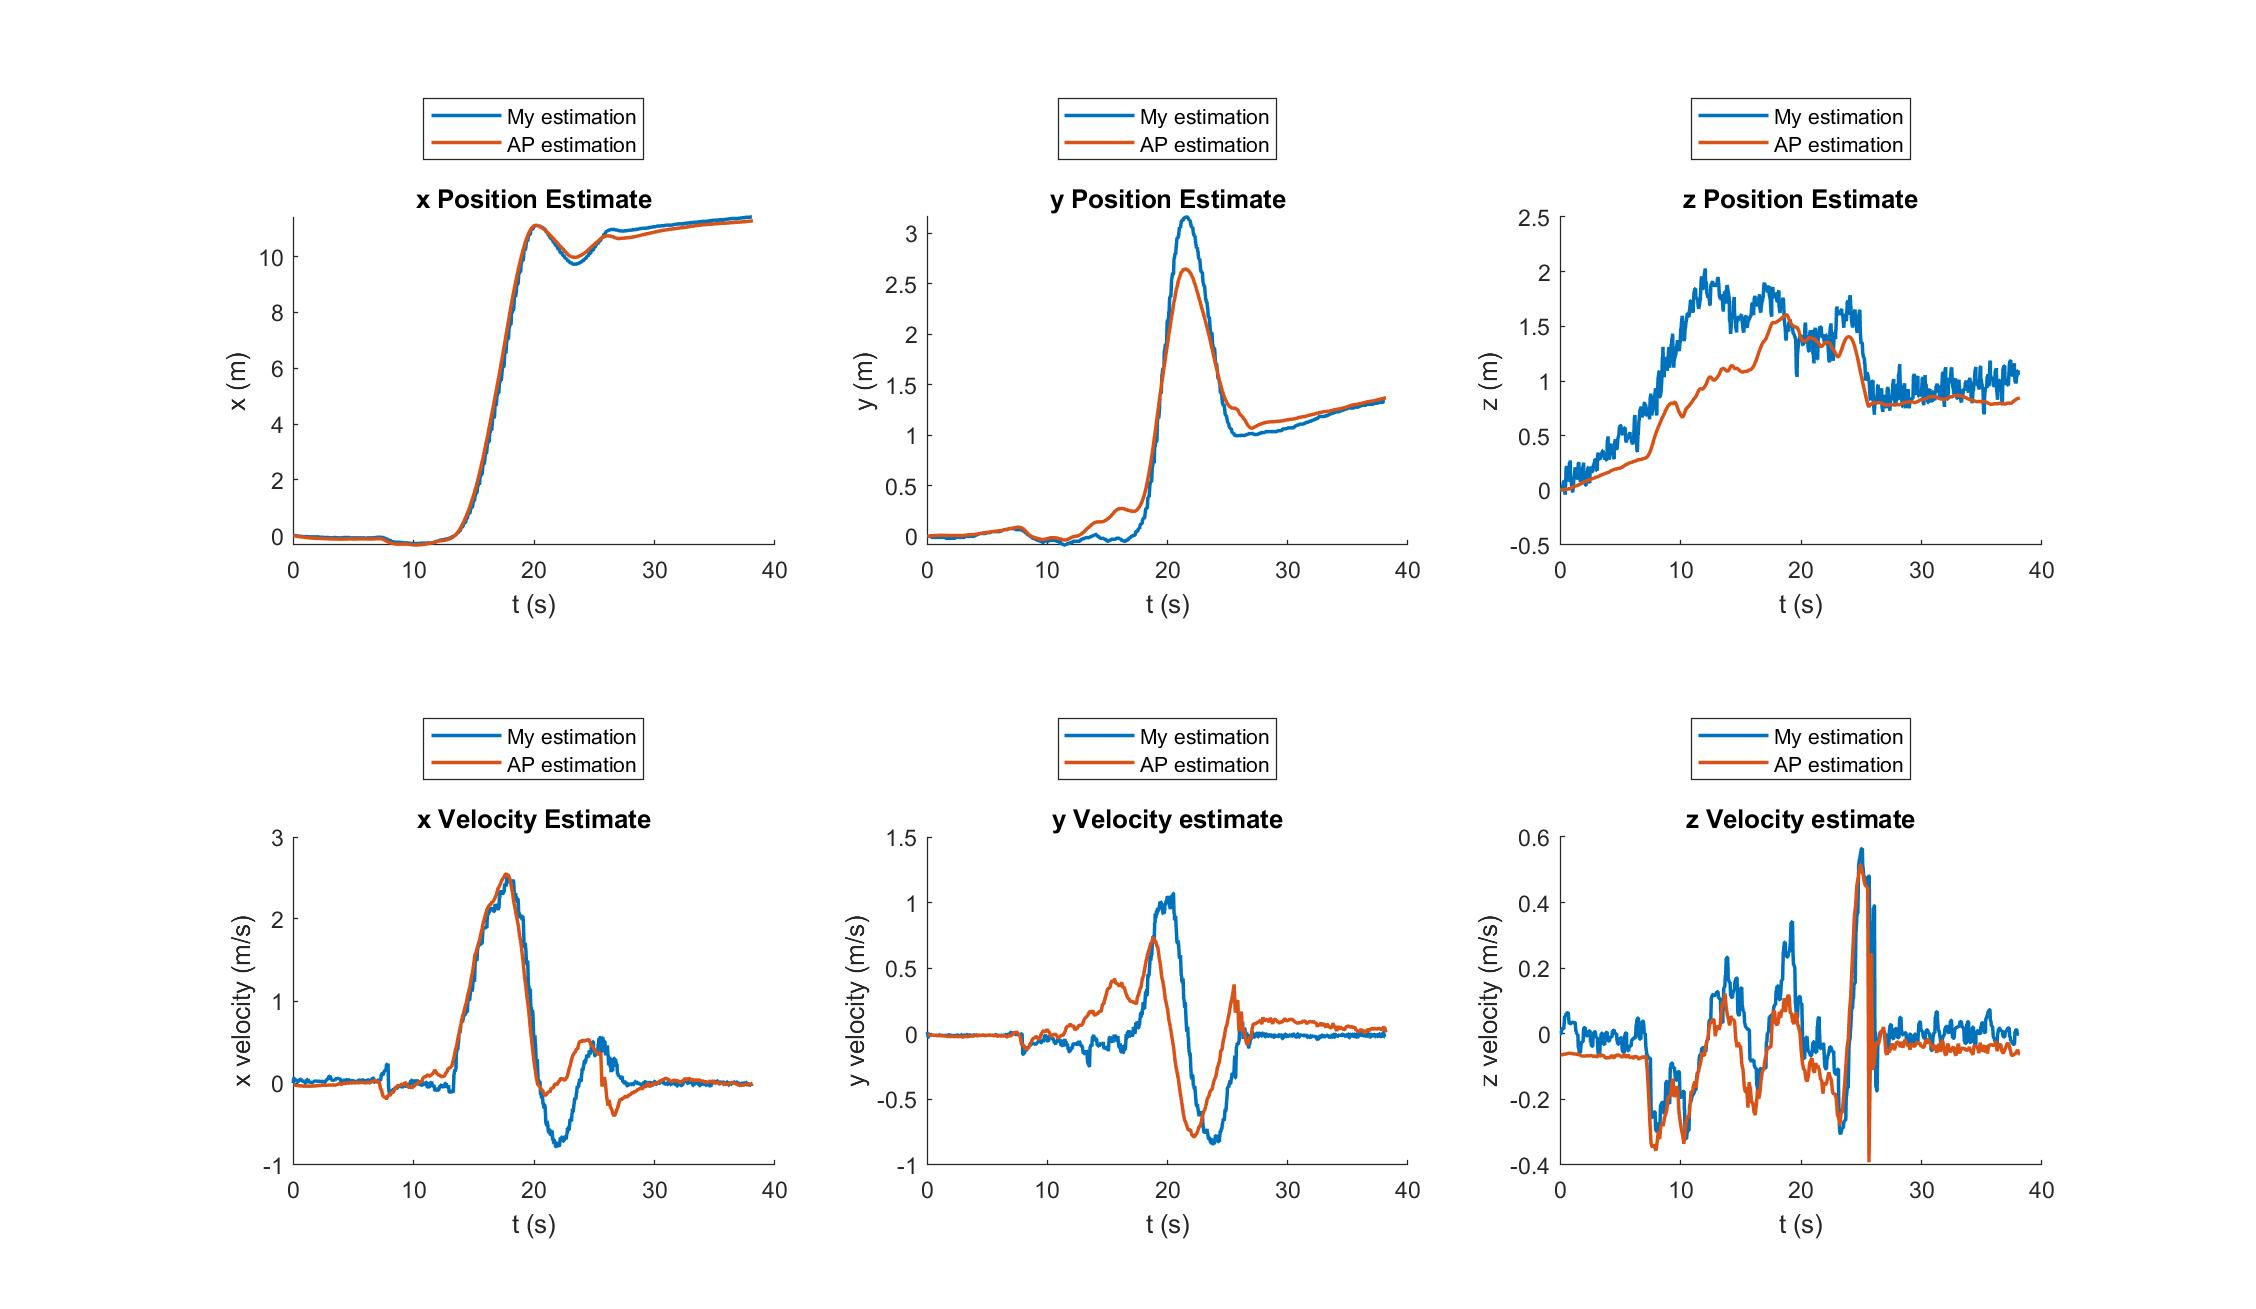
\includegraphics[width=\columnwidth]{EKF_HW/GPS/FlightTest1_Pos.jpg}%
	\caption{The EKF position and velocity estimates compared with the ArduPilot EKF estimates for flight test \#1.}%
	\label{fig:HW_GPS_Pos}%
\end{figure}

\begin{figure}[htb]
	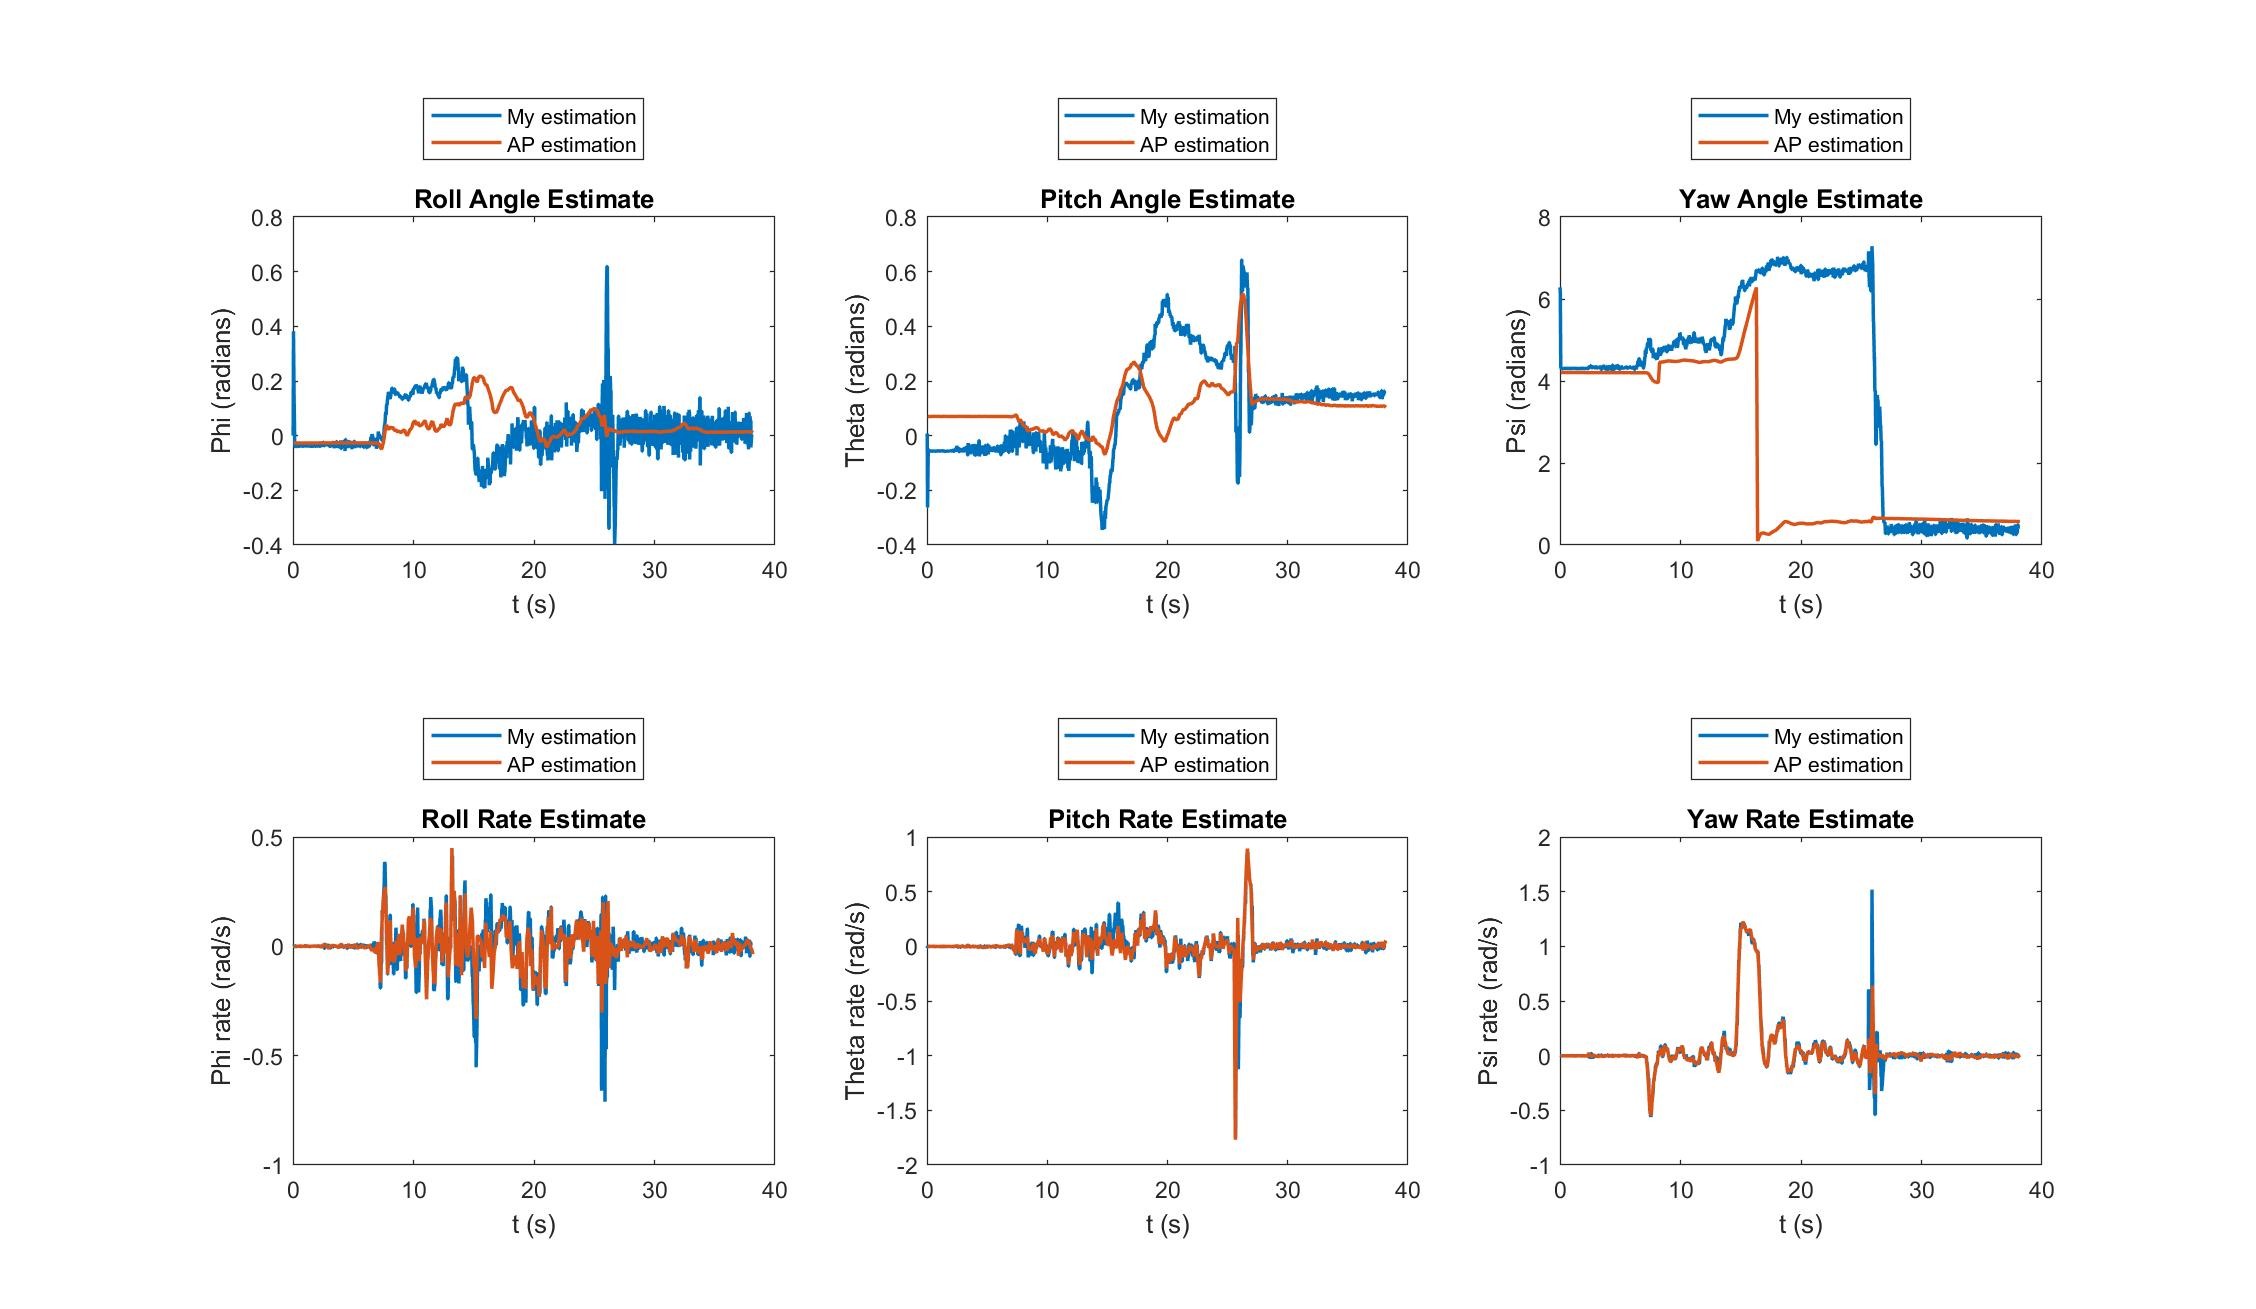
\includegraphics[width=\columnwidth]{EKF_HW/GPS/FlightTest1_Angle.jpg}%
	\caption{The EKF angular estimates compared with the ArduPilot EKF estimates for flight test \#1.}%
	\label{fig:HW_GPS_Ang}%
\end{figure}

A flight test was then repeated with the optical flow sensor installed, in order to evaluate the effectiveness of the EKF in the absence of GPS data. This flight involved taking off to a height off approximately 1.5 m, hovering at that point for approximately 10 seconds and then landing at the same point. The results of the EKF are shown in \figref{fig:HW_OFS_Pos}, compared with the AP estimation (which uses GPS data). The position and velocity estimates are not extremely accurate, however it can be seen that there is no significant drift in the position estimates over this time period.

\begin{figure}[htb]
	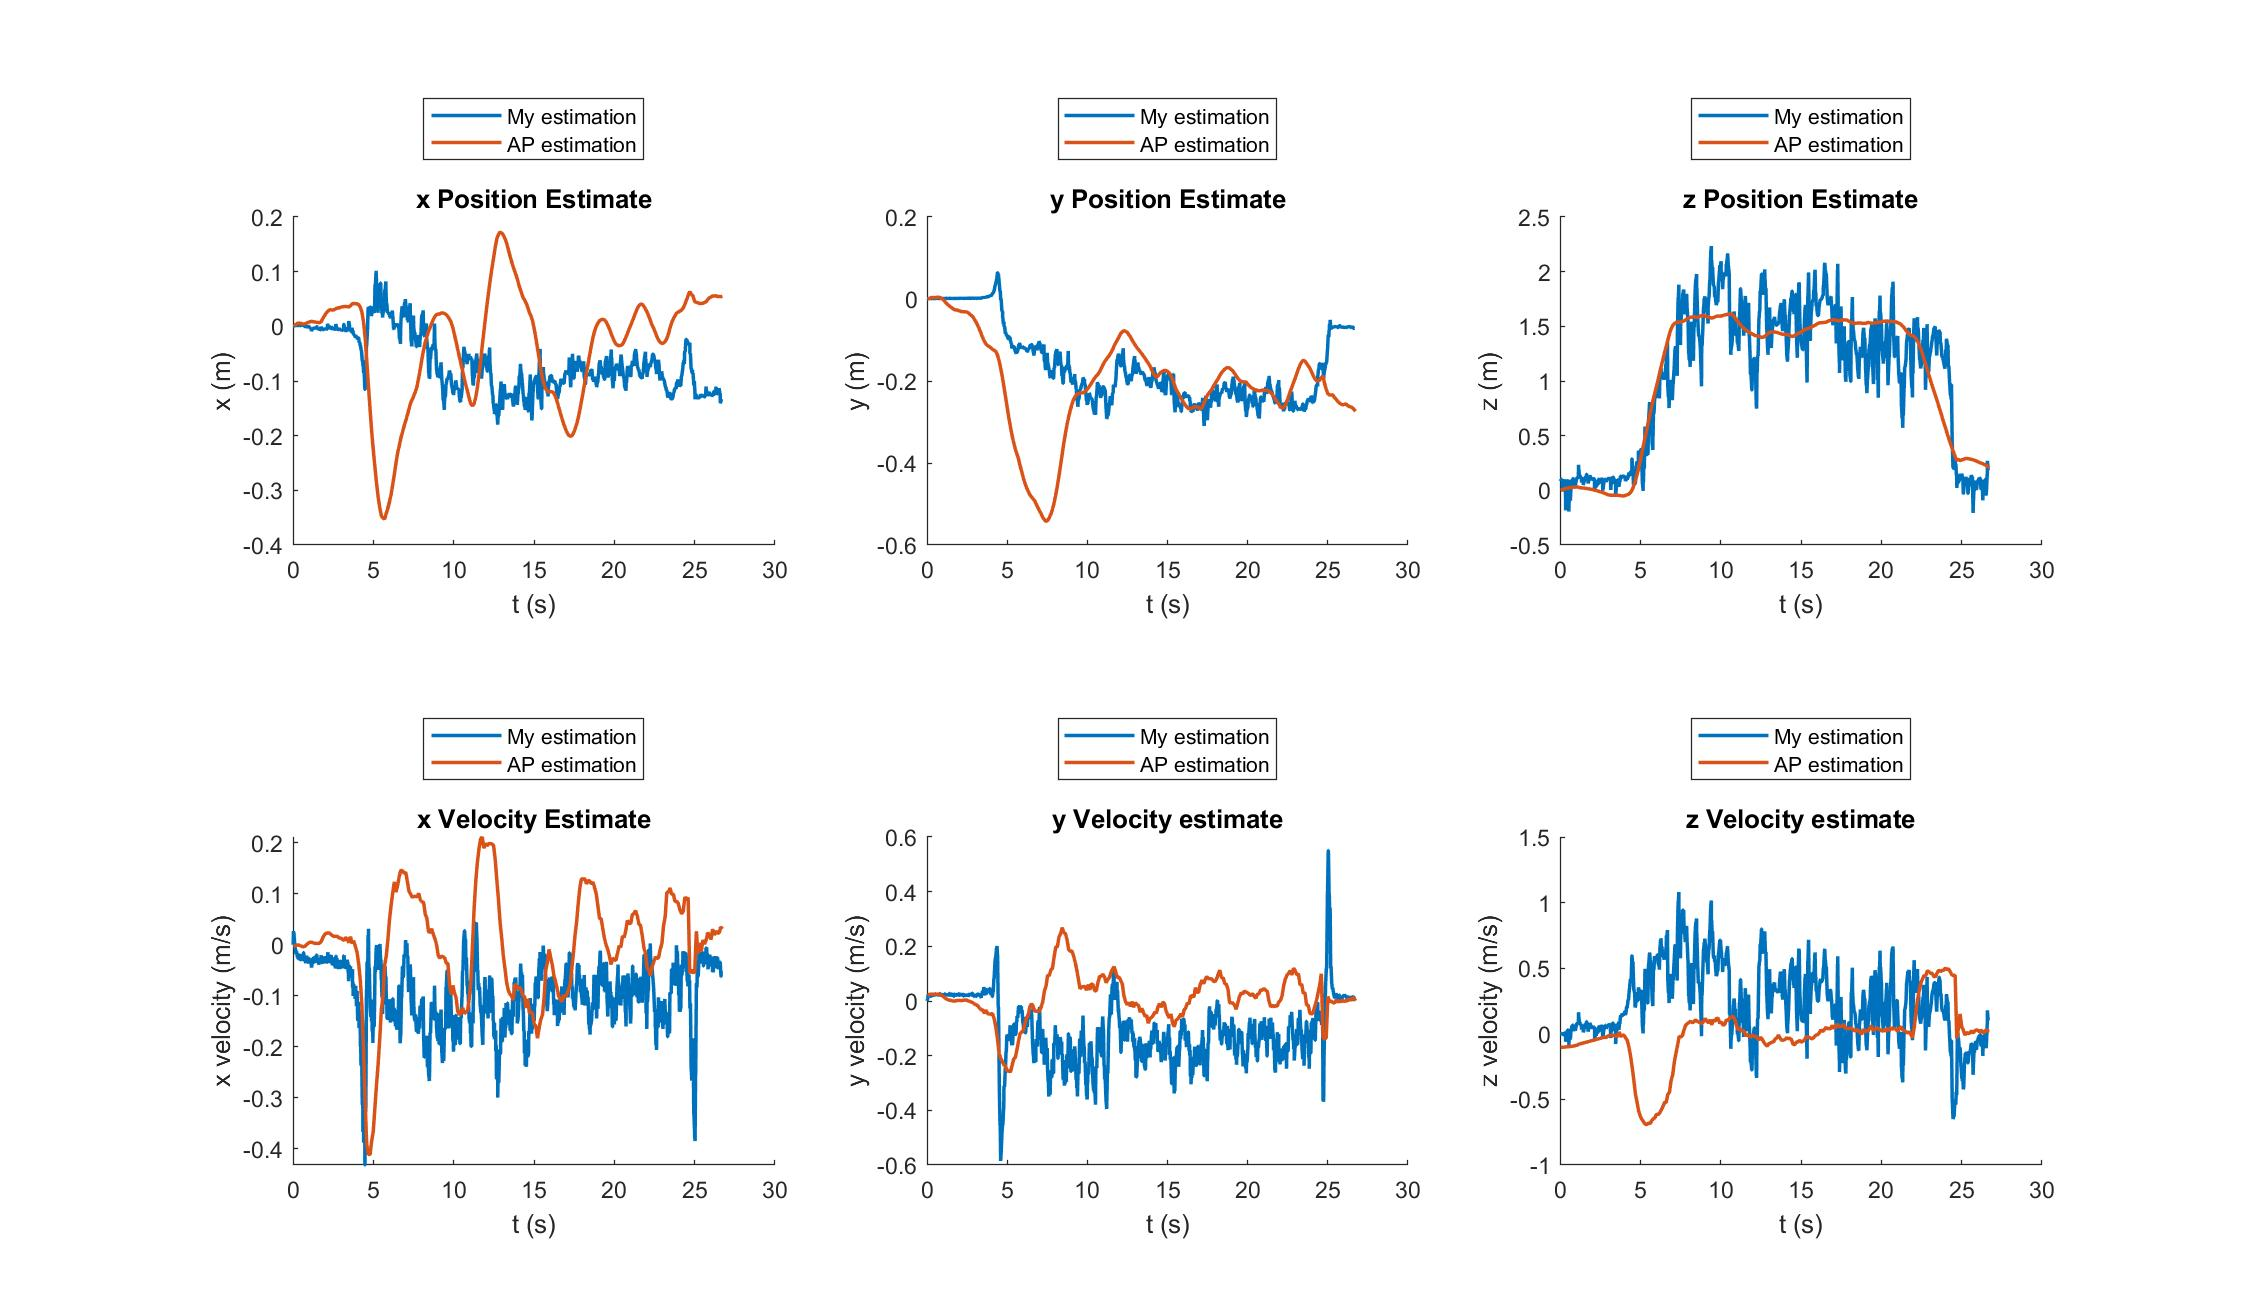
\includegraphics[width=\columnwidth]{EKF_HW/OFS/FlightTest2_Pos.jpg}%
	\caption{The OFS EKF position and velocity estimates compared with the ArduPilot EKF estimates for flight test \#2.}%
	\label{fig:HW_OFS_Pos}%
\end{figure}

A third flight was undertaken in which the aircraft was programmed to take off to 1.5m, hover in place for 10 seconds, then travel some distance to land at another waypoint. This flight resulted in a collision with the ground (likely due to unreliable lidar data), however the first 25 seconds of data was able to be used for analysis. Using this data, it could be seen that using the OFS data alone was insufficient for tracking positional change. 

\FloatBarrier
\subsection{Discussion of Results}
To produce these results, the sensor data that was recorded on the SD card was processed post-flight in MATLAB. It is important to note that the data which is recorded on the SD card is not representative of all of the sensor data available to the flight controller. That is, the flight controller samples the sensors at a faster rate and not all data is logged. This severely limits the accuracy of the estimated states which are based upon this data. For example, the IMU is sampled at a rate of at least 1 kHz, however the data is logged at a rate of approximately 25 Hz. This issue was particularly prominent for the optical flow sensor data, which was logged at a rate of only 10 Hz but has a capability of 121 Hz. If the EKF was run directly on the hardware it may prove to be more accurate. \\

Another issue that arose was the unreliability of the lidar data. The datasheet states that the sensor only has an operating range of 2 m. Although, the flight test was conducted at 1.5 m above the ground, the angle of the vehicle during translational motion presumably caused the lidar line of sight to ground to exceed 2 m. This resulted in the lidar being unable to record data and therefore impacting the accuracy of the results - since the optical flow velocity estimates rely on knowledge of the scene depth. The operating range of this sensor makes it essentially useless for practical flights. However there are many other commercially available lidar sensors with larger operating ranges. Alternatively, many optical flow sensors are instead paired with sonar (ultrasonic) sensors for scene depth information.



\section{Chapter Summary}
This chapter introduced the hexacopter platform's hardware and software architecture. A number of flight tests were carried out and the data was processed post-flight using the previously developed EKF algorithms. It is shown that with the particular optical flow sensor that was chosen, position data was not able to be accurately estimated during motion.

\clearpage


